%Version 3.1 December 2024
% See section 11 of the User Manual for version history
%
%%%%%%%%%%%%%%%%%%%%%%%%%%%%%%%%%%%%%%%%%%%%%%%%%%%%%%%%%%%%%%%%%%%%%%
%%                                                                 %%
%% Please do not use \input{...} to include other tex files.       %%
%% Submit your LaTeX manuscript as one .tex document.              %%
%%                                                                 %%
%% All additional figures and files should be attached             %%
%% separately and not embedded in the \TeX\ document itself.       %%
%%                                                                 %%
%%%%%%%%%%%%%%%%%%%%%%%%%%%%%%%%%%%%%%%%%%%%%%%%%%%%%%%%%%%%%%%%%%%%%

%%\documentclass[referee,sn-basic]{sn-jnl}% referee option is meant for double line spacing

%%=======================================================%%
%% to print line numbers in the margin use lineno option %%
%%=======================================================%%

%%\documentclass[lineno,pdflatex,sn-basic]{sn-jnl}% Basic Springer Nature Reference Style/Chemistry Reference Style

%%=========================================================================================%%
%% the documentclass is set to pdflatex as default. You can delete it if not appropriate.  %%
%%=========================================================================================%%

%%\documentclass[sn-basic]{sn-jnl}% Basic Springer Nature Reference Style/Chemistry Reference Style

%%Note: the following reference styles support Namedate and Numbered referencing. By default the style follows the most common style. To switch between the options you can add or remove �Numbered� in the optional parenthesis. 
%%The option is available for: sn-basic.bst, sn-chicago.bst%  
 
%%\documentclass[pdflatex,sn-nature]{sn-jnl}% Style for submissions to Nature Portfolio journals
%%\documentclass[pdflatex,sn-basic]{sn-jnl}% Basic Springer Nature Reference Style/Chemistry Reference Style
\documentclass[pdflatex,sn-mathphys-num]{sn-jnl}% Math and Physical Sciences Numbered Reference Style
%%\documentclass[pdflatex,sn-mathphys-ay]{sn-jnl}% Math and Physical Sciences Author Year Reference Style



%%\documentclass[pdflatex,sn-aps]{sn-jnl}% American Physical Society (APS) Reference Style
%%\documentclass[pdflatex,sn-vancouver-num]{sn-jnl}% Vancouver Numbered Reference Style
%%\documentclass[pdflatex,sn-vancouver-ay]{sn-jnl}% Vancouver Author Year Reference Style
%%\documentclass[pdflatex,sn-apa]{sn-jnl}% APA Reference Style
%%\documentclass[pdflatex,sn-chicago]{sn-jnl}% Chicago-based Humanities Reference Style

%%%% Standard Packages
%%<additional latex packages if required can be included here>
% 设置中文


\RequirePackage{etex}

\usepackage[UTF8]{ctex}
% \usepackage{xeCJK}
% \setCJKmainfont{Noto Serif CJK SC}
% \usepackage{unicode-math}   % 替代 amssymb + bm + fontspec

\usepackage{subfigure}
\usepackage{tabularx}
\usepackage{graphicx}
\usepackage{float}
\usepackage{epstopdf}
\usepackage{microtype}
\usepackage{enumitem}
\usepackage{multirow}
\usepackage{bbding}
\usepackage{amsmath}
% \usepackage{color}
\usepackage{bm}
\usepackage{cleveref}  
% \usepackage[authoryear,sort&compress,longnamesfirst]{natbib}
\usepackage{xcolor}
\usepackage{hyperref}
\usepackage{amssymb} 
\usepackage{amsthm} 
\usepackage{booktabs}
%%%%
% 可选:让 epstopdf 自动在 \includegraphics 时启用
\epstopdfsetup{outdir=./}
%%%%%=============================================================================%%%%
%%%%  Remarks: This template is provided to aid authors with the preparation
%%%%  of original research articles intended for submission to journals published 
%%%%  by Springer Nature. The guidance has been prepared in partnership with 
%%%%  production teams to conform to Springer Nature technical requirements. 
%%%%  Editorial and presentation requirements differ among journal portfolios and 
%%%%  research disciplines. You may find sections in this template are irrelevant 
%%%%  to your work and are empowered to omit any such section if allowed by the 
%%%%  journal you intend to submit to. The submission guidelines and policies 
%%%%  of the journal take precedence. A detailed User Manual is available in the 
%%%%  template package for technical guidance.
%%%%%=============================================================================%%%%

%% as per the requirement new theorem styles can be included as shown below
\theoremstyle{thmstyleone}%
\newtheorem{theorem}{Theorem}%  meant for continuous numbers
%%\newtheorem{theorem}{Theorem}[section]% meant for sectionwise numbers
%% optional argument [theorem] produces theorem numbering sequence instead of independent numbers for Proposition
\newtheorem{proposition}[theorem]{Proposition}% 
%%\newtheorem{proposition}{Proposition}% to get separate numbers for theorem and proposition etc.
\newtheorem{lemma}{Lemma}[section] 
\newtheorem{assumption}{Assumption}
\theoremstyle{thmstyletwo}%
\newtheorem{example}{Example}%
\newtheorem{remark}{Remark}%

\theoremstyle{thmstylethree}%
\newtheorem{definition}{Definition}%

\raggedbottom
%%\unnumbered% uncomment this for unnumbered level heads

\begin{document}

\title[Article Title]{Predefined Time Prescribed Performance Backstepping Control for Robotic Manipulators with Input Saturation}

%%=============================================================%%
%% GivenName	-> \fnm{Joergen W.}
%% Particle	-> \spfx{van der} -> surname prefix
%% FamilyName	-> \sur{Ploeg}
%% Suffix	-> \sfx{IV}
%% \author*[1,2]{\fnm{Joergen W.} \spfx{van der} \sur{Ploeg} 
%%  \sfx{IV}}\email{iauthor@gmail.com}
%%=============================================================%%

\author[1,2]{\fnm{} \sur{Shuli Liu}}\email{shunnee@163.com}
% \credit{Writing - Original Draft, Methodology, Software, Visualization, Data curation}


\author*[3]{\fnm{} \sur{Yi Liu}}\email{liuyi_hust@163.com}
\author*[3]{\fnm{} \sur{Jingang Liu}}\email{wellbuild@126.com}
% \credit{Resources, Investigation, Formal analysis, Conceptualization, Writing - Review \& Editing}
% \equalcont{These authors contributed equally to this work.}

% \credit{Project administration, Validation, Funding acquisition, Writing - Review \& Editing}
% \equalcont{These authors contributed equally to this work.}
\author*[1,2]{\fnm{} \sur{Yin Yang}}\email{yangyinxtu@xtu.edu.cn}
% \credit{Supervision, Funding acquisition, Writing - Review \& Editing}
% \equalcont{These authors contributed equally to this work.}

\affil[1]{\orgname{School of Mathematics and Computational Science, Xiangtan University}, \orgaddress{\street{Street}, \city{City}, \postcode{411105}, \country{China}}}

\affil[2]{\orgname{National Center for Applied Mathematics in Hunan}, \orgaddress{\street{Street}, \city{City}, \postcode{411105}, \country{China}}}

\affil[3]{\orgname{School of Mechanical Engineering and Mechanics, Xiangtan University}, \orgaddress{\street{Street}, \city{City}, \postcode{411105}, \country{China}}}



% Here goes the abstract
\abstract{
% To simultaneously address the challenges of uncontrollable convergence time and the difficulty of unifying performance constraints in trajectory tracking control for uncertain nonlinear robotic manipulators, this paper proposes a novel adaptive control framework that integrates predefined-time convergence with prescribed performance constraints. Specifically, a new class of Bernstein-polynomial-based performance functions is designed to achieve smooth and adjustable boundaries for both position and velocity errors, significantly reducing dependence on initial error conditions. An exponential barrier Lyapunov function is further introduced to strictly constrain the entire error evolution process. The controller is constructed using the backstepping method and incorporates a radial basis function neural network for online compensation of unknown nonlinear dynamics, thereby enhancing the system’s adaptability and robustness. The proposed approach organically combines predefined-time stability theory with dynamic performance regulation, theoretically guaranteeing the uniform boundedness of all closed-loop signals and prescribed-time convergence of the tracking error. Finally, simulation and experimental verification are carried out on a typical two-degree-of-freedom robotic arm system and a real six-degree-of-freedom collaborative robot platform. The results show that the proposed method outperforms existing schemes in terms of tracking accuracy, convergence speed and robustness, and is particularly suitable for high-performance and time-sensitive robotic systems.
本文研究了具有未知动力学、有界扰动以及执行器饱和条件下的机器人机械臂轨迹跟踪控制问题,提出了一种立于任何初始状态条件的预定义时间预设性能约束的自适应反步控制方法。针对传统预设性能控制中存在的初值奇异性和误差变换非光滑问题,针对每个通道独立设计了结合多项式性能函数与误差缩放函数的预定义时间误差变换结构,确保系统状态在预定义时间内严格且平滑地满足全局预设性能约束。
为处理反步控制及执行器饱和输入引起的计算复杂度爆炸问题,设计了一种预定义时间饱和补偿器,以同时消除命令滤波与输入饱和的不利影响。此外,引入一阶滑模扰动观测器实时估计并补偿系统中未知的有界扰动,利用径向基函数神经网络对系统未建模动态进行辨识和补偿,从而提高了控制系统的鲁棒性和跟踪精度。同时,结合预定义时间理论和自适应动态障碍李雅普诺夫函数,严格证明了闭环系统在预定义时间内的全局稳定性和误差收敛性。
数值和实验结果结果验证了所提出方法的有效性,与现有方法相比,本文方法在响应速度、稳态精度及鲁棒性能方面表现出明显优势。

}
\keywords{Prescribed performance control, predefined-time stability, adaptive dynamic barrier Lyapunov function, backstepping control, input saturation, robotic manipulators' trajectory tracking.
}
\maketitle

% Main text

下面是在你原有排版基础上**逐句打磨、修正符号与措辞**后的版本(保留结构与编号;只做必要的更正与增润)。

---

\subsection{System description}






\begin{lemma} \label{lemma:1} (Predefined-time stability \cite{WangEtAl_2022_Adaptivefuzzy}).
	Consider the system $\dot{x}(t)=f(x(t))$ with $x(0)=x_0$, where $x\in\mathbb{R}^n$ is the state. The vector field $f(\cdot)$ is continuous and satisfies $f(0)=0$.
	%
	Let $V:\mathbb{R}^n\to\mathbb{R}_+$ be continuously differentiable, positive definite, and radially unbounded, with $V(0)=0$ and $V(x)>0$ for all $x\neq 0$.
	For given design parameters $0<\eta<1$, $T_p>0$, and $0<\varsigma<\infty$, suppose the closed-loop system satisfies
	\begin{equation}\label{eq:7}
	  \dot V(x)\;\le\;
	  -\frac{\pi}{\eta T_p}\Big(V(x)^{\,1-\frac{\eta}{2}}+V(x)^{\,1+\frac{\eta}{2}}\Big)
	  +\varsigma .
	\end{equation}
	Then the origin is predefined-time stable with convergence time bounded by $T_p$. Moreover,
	\begin{equation}\label{eq:8}
	  V(T_p)\;\le\;
	  \min\!\left\{
		\Big(\tfrac{\eta T_p\,\varsigma}{\pi}\Big)^{\!\frac{1}{\,1-\frac{\eta}{2}\,}},
		\;
		\Big(\tfrac{\eta T_p\,\varsigma}{\pi}\Big)^{\!\frac{1}{\,1+\frac{\eta}{2}\,}}
	  \right\}.
	\end{equation}
	In particular, if $\varsigma=0$ then $V(T_p)=0$.
	\end{lemma}
	
	\begin{lemma}\label{lemma:2} \cite{TeeEtAl_2009_Barrierlyapunova}
	For $\mathcal{X},\mathcal{Y}\ge 0$ and exponents $\mathcal{Z}_1,\mathcal{Z}_2>1$ with $\tfrac{1}{\mathcal{Z}_1}+\tfrac{1}{\mathcal{Z}_2}=1$, the Young inequality holds:
	\begin{equation}\label{eq:9}
	  \mathcal{X}\,\mathcal{Y}\;\le\;\frac{\mathcal{X}^{\mathcal{Z}_1}}{\mathcal{Z}_1}
	  +\frac{\mathcal{Y}^{\mathcal{Z}_2}}{\mathcal{Z}_2}.
	\end{equation}
	Moreover, for any $\mathcal{Z}_{1},\mathcal{Z}_{2}>0$ with $\mathcal{Z}_{1}+\mathcal{Z}_{2}=1$ and any $\mathcal{Z}_{3}>0$ (generalized weighted form),
	\begin{equation}\label{eq:10}
	  |\mathcal{X}|^{\mathcal{Z}_{1}}\,|\mathcal{Y}|^{\mathcal{Z}_{2}}
	  \;\le\;
	  \mathcal{Z}_{1}\,\mathcal{Z}_{3}^{-\frac{\mathcal{Z}_{2}}{\mathcal{Z}_{1}}}\,|\mathcal{X}|
	  +\mathcal{Z}_{2}\,\mathcal{Z}_{3}\,|\mathcal{Y}|.
	\end{equation}
	\end{lemma}
	
	\begin{lemma}\label{lemma:3} \cite{HardyLittlewoodPolya_1952_Inequalities}
	Let $\mathcal{X}_i\in\mathbb{R}$ and $\mathcal{Y}\in\mathbb{R}^+$. Then
	\begin{equation}\label{eq:11}
	  \sum_{i=1}^{n}|\mathcal{X}_i|^{\mathcal{Y}}
	  \;\ge\;
	  \Big(\sum_{i=1}^{n}|\mathcal{X}_i|\Big)^{\mathcal{Y}},\qquad \mathcal{Y}\in(0,1),
	\end{equation}
	and
	\begin{equation}\label{eq:12}
	  \sum_{i=1}^{n}|\mathcal{X}_i|^{\mathcal{Y}}
	  \;\ge\;
	  n^{\,1-\mathcal{Y}}\Big(\sum_{i=1}^{n}|\mathcal{X}_i|\Big)^{\mathcal{Y}},
	  \qquad \mathcal{Y}\in(1,\infty).
	\end{equation}
	\end{lemma}
	
	\begin{lemma}\label{lemma:4} \cite{TeeEtAl_2009_Barrierlyapunov}
	For $\mathcal{Y}>0$ and $\mathcal{X}\in\mathbb{R}$ with $|\mathcal{X}|<\mathcal{Y}$, it holds that
	\begin{equation}\label{eq:13}
	  \log\!\Big(\frac{\mathcal{Y}^{2}}{\mathcal{Y}^{2}-\mathcal{X}^{2}}\Big)
	  \;\le\;
	  \frac{\mathcal{X}^{2}}{\mathcal{Y}^{2}-\mathcal{X}^{2}}.
	\end{equation}
	\end{lemma}
	


	\section{Predefined time error transformation function}

	为同时化解初值越界奇异性、实现全局动态误差约束,并保证轨迹误差在预定义时间内按可调路径被合法压缩与稳定收敛,本文提出由\emph{性能函数} $\rho(t)$、\emph{误差缩放函数} $\beta(t)$ 与\emph{缩放误差} $z(t)$ 组成的预定义时间误差变换结构。
	
	\paragraph{性能函数(Bernstein 形状调制)}
	\begin{equation}\label{eq:14}
	  \rho(t) = a + \big(\rho_0 - a\big)\sum_{i=0}^4 \nu_i B_{i,4}(b), 
	  \qquad \nu_0 = 1 > \nu_1 > \cdots > \nu_4 = 0,
	\end{equation}
	其中 $b = \big(t/T_p\big)^{p}\in[0,1]$ 为归一化时间,$T_p>0$ 为预定义收敛时间,$0<p<1$ 用于加快初期压缩速率;$\rho_0$ 与 $a$ 分别为初始与稳态误差上界。四次 Bernstein 基函数满足 $\sum_{i=0}^{4} B_{i,4}(b)=1,\ 0\le B_{i,4}(b)\le 1$。
	
	由 \cref{eq:14} 可得 $\rho(t)$ 的性质:  
	1) 端点与连续性:$\rho(0)=\rho_0,\ \rho(T_p^-)=\rho(T_p^+)=a$(令 $t\ge T_p$ 时 $\rho(t)\equiv a$)。  
	2) 单调性:因 $\nu_0>\cdots>\nu_4$ 且 $b$ 单增,$\rho(t)$ 严格单调递减,$\dot\rho(t)<0$。  
	3) 光滑性:$\rho(t)$ 在 $[0,\infty)$ 上连续可导。其导数为
	\begin{equation}\label{eq:15}
	  \dot{\rho}(t)
	  \;=\; 4\big(\rho_0 - a\big)\!\sum_{i=0}^{3}\!\big(\nu_{i+1}-\nu_i\big)\,B_{i,3}(b)\,\dot b,
	  \qquad 
	  \dot b=\frac{p}{T_p}\Big(\frac{t}{T_p}\Big)^{p-1}>0,
	\end{equation}
	等价地写成 $-\!4(\rho_0-a)\sum_{i=0}^{3}(\nu_i-\nu_{i+1})B_{i,3}(b)\dot b$,以显式呈现负号(两式等价;原稿遗漏了系数 $4$,已补全)。
	
	\paragraph{误差缩放函数(正则不完全 Beta 形状器)}
	为实现对误差“先缓后急/先急后缓”等可调缩放,定义
	\begin{equation}\label{eq:16}
	  \beta(t)=
	  \begin{cases}
		\displaystyle \dfrac{1}{I(\upsilon_{1},\upsilon_{2})}\!\int_{0}^{b}\! u^{\upsilon_{1}-1}(1-u)^{\upsilon_{2}-1}\,du, & t\in[0,T_p),\\[8pt]
		1, & t\in[T_p,\infty),
	  \end{cases}
	\end{equation}
	其中 $\upsilon_{1}>1,\ \upsilon_{2}>1$ 为形状参数,$I(\upsilon_{1},\upsilon_{2})=\int_{0}^{1}u^{\upsilon_{1}-1}(1-u)^{\upsilon_{2}-1}du$ 为归一化因子,使得 $\beta:[0,T_p)\!\to[0,1]$。由定义得
	\begin{subequations}\label{eq:17}
	\begin{align}
	  &\lim_{t\to T_p^-}\beta(t)=\lim_{t\to T_p^+}\beta(t)=1,\\
	  &\lim_{t\to T_p^-}\dot\beta(t)=\lim_{t\to T_p^+}\dot\beta(t)=0,
	\end{align}
	\end{subequations}
	其中 $t\!\to\!T_p^-$ 时,因 $(1-b)^{\upsilon_2-1}\!\to\!0$($\upsilon_2\!>\!1$),导数自然趋零。$\beta(t)$ 的显式导数为
	\begin{equation}\label{eq:18}
	  \dot\beta(t)=
	  \begin{cases}
		\dfrac{1}{I(\upsilon_{1},\upsilon_{2})}\ \dot b\ b^{\upsilon_{1}-1}(1-b)^{\upsilon_{2}-1}, & t\in[0,T_p),\\[6pt]
		0, & t\in[T_p,\infty).
	  \end{cases}
	\end{equation}
	由此可见:1) $\beta(0)=0,\ \beta(T_p)=1$;2) $\dot\beta(t)>0$,$\beta(t)$ 严格单增;3) $\beta$ 在 $[0,\infty)$ 上 $C^1$(在 $t=T_p$ 左右导数一致为 $0$)。
	
	\paragraph{缩放误差与可行性保障}
	定义缩放误差
	\begin{equation}\label{eq:19}
	  z(t)=\beta(t)\,e(t), \qquad t\in[0,T_p),
	\end{equation}
	其中 $e(t)$ 为原始跟踪误差。该构造满足:  
	1) $z(0)=0<\rho_0$,即便 $|e(0)|>\rho(0)$ 也保证 Lyapunov 初值有限并\emph{避免初值奇异性};  
	2) 受控下的约束被转写为 $|z(t)|<\rho(t)$($\beta\!\in\![0,1]$ 将超界误差即时“合法化”,随后由控制律保持可行);  
	3) 当 $t\ge T_p$ 时 $\beta(t)=1,\ \rho(t)=a$,约束自然退化为稳态精度界 $|e(t)|<a$。
	
	\begin{figure}[H]
	  \centering
	  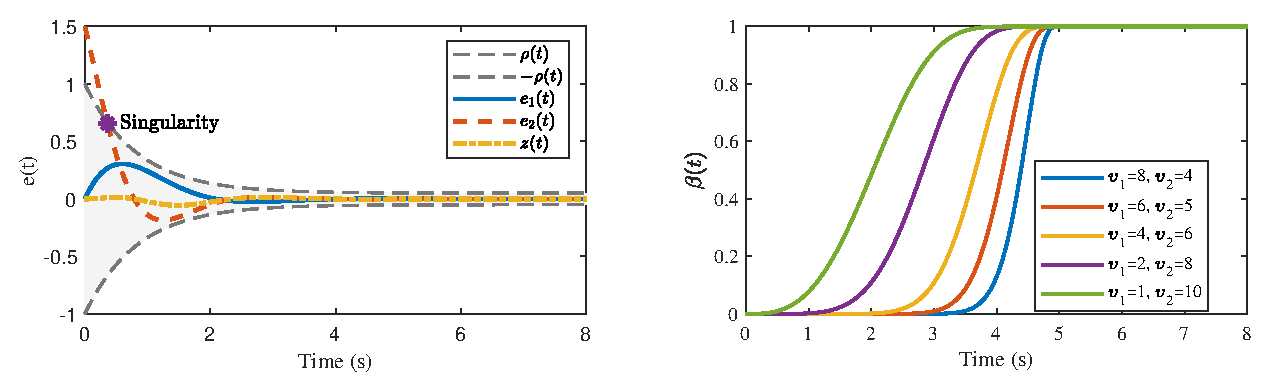
\includegraphics[width=0.9\textwidth]{fig1.eps}
	  \caption{Error shift transformation and shape-tunable shift function. 第一幅展示了经变换后的(合法化的)误差轨迹 $z(t)$;第二幅展示不同 $(\upsilon_1,\upsilon_2)$ 下 $\beta(t)$ 的形状可调性(早期更平/更陡),体现“力矩峰值—收敛速度—稳态精度”的权衡可调。}
	  \label{fig:1}
	\end{figure}
	
	\begin{remark}[本节结构的创新点与优势]
	\leavevmode
	\begin{itemize}
	  \item \textbf{初值可行性—从源头消除奇异性}:传统 PPC 以 $z=e/\rho$ 变换,若 $|e(0)|>\rho(0)$ 即落入非法区,需额外机制修正;本文以 $\beta(0)=0$ 强制 $z(0)=0$,\emph{变量层面}直接规避初值奇异性。
	  \item \textbf{预定义时间与可调路径并重}:$\rho(t)$(Bernstein 加权)与 $\beta(t)$(正则不完全 Beta)分别单调收紧/放宽有效域与缩放强度,$T_p$、$\{\nu_i\}$、$p$、$(\upsilon_1,\upsilon_2)$ 组成\emph{互补调谐器}:前者控制“边界收紧节奏”,后者控制“误差注入强度”,从而把“预定义时间 + 预设性能”的\emph{收敛路径}做成\emph{可设计}对象。
	  \item \textbf{闭式导数,控制器友好}:$\dot\rho(t)$ 与 $\dot\beta(t)$ 具备\emph{封闭、光滑、可界}的解析表达(见 \cref{eq:15,eq:18}),可无缝嵌入 Lyapunov/backstepping/SMC 等推导,避免对数/有理型 BLF 常见的导数复杂与不可控问题。
	  \item \textbf{执行器友好性}:通过 $(\upsilon_1,\upsilon_2)$ 形状调制,可以在早期降低攻顶力度(抑制力矩峰值),在后期提高压缩速率(提升稳态精度),实现\emph{性能—能耗—饱和}的三方折中。
	  \item \textbf{普适可扩展}:该 $(\rho,\beta,z)$ 架构不依赖具体动态模型细节,可直接用于反步、自适应、滑模与容错控制等多类非线性框架,并可与饱和补偿、NN/RBF 估计等模块级联。
	\end{itemize}
	\end{remark}




	下面是在你原有**结构与编号**基础上,逐句校对并强化“创新点”的可直接替换版(仅对措辞、符号、自洽性与交叉引用做必要修订):

	---
	
	\section{Main results}
	
	In this section, we develop a backstepping–BLF controller that enforces **predefined-time convergence** together with **prescribed performance**. The overall architecture is illustrated in \cref{fig:1}.
	
	\par For trajectory tracking, define the error signals
	\begin{subequations}\label{eq:20}
	\begin{align}
	\&e_{1}=x_{1}-x_{d}-\zeta_{1},\\
	\&e_{2}=x_{2}-\alpha^{f}-\zeta_{2},
	\end{align}
	\end{subequations}
	where $\alpha$ is the virtual control, $\operatorname{sat}(\alpha)$ denotes its elementwise saturation, $\alpha^{f}$ is a filtered version of $\operatorname{sat}(\alpha)$, and $\zeta_{1},\zeta_{2}\in\mathbb{R}^{n}$ are **dynamic anti-saturation compensators** (virtual and actual channels, respectively).
	
	\subsection{预定义时间饱和补偿器构造}
	
	\noindent\textbf{Virtual-input saturation residue.} Define the virtual saturation residue (difference between the commanded and saturated signals)
	\begin{equation}\label{eq:21}
	\Delta \alpha_{i}\triangleq \alpha_{i}-\operatorname{sat}(\alpha_{i})=
	\begin{cases}
	\alpha_{i}-\alpha_{\max}, & \alpha_{i}\ge \alpha_{\max},\\
	0,                        & \alpha_{\min}<\alpha_{i}<\alpha_{\max},\\
	\alpha_{i}-\alpha_{\min}, & \alpha_{i}\le \alpha_{\min},
	\end{cases}
	\end{equation}
	where $\alpha_{\max},\alpha_{\min}$ are the bounds of the virtual input.
	
	\noindent\textbf{Filter for $\operatorname{sat}(\alpha)$.} To smooth $\operatorname{sat}(\alpha)$ and facilitate Lyapunov design, introduce
	\begin{equation}\label{eq:22}
	\dot{\alpha}^{f}=-\lambda\big(\alpha^{f}-\operatorname{sat}(\alpha)\big),\qquad
	\alpha^{f}(0)=\operatorname{sat}(\alpha)(0),
	\end{equation}
	with bandwidth $\lambda>1$. Define the filter mismatch
	\begin{equation}\label{eq:23}
	\tilde{\alpha}\triangleq \operatorname{sat}(\alpha)-\alpha^{f}.
	\end{equation}
	From \cref{eq:22}, its dynamics satisfy
	
	$$
	  \dot{\tilde{\alpha}}=\dot{\operatorname{sat}}(\alpha)-\dot{\alpha}^{f}
	  \,=\,\dot{\operatorname{sat}}(\alpha)-\lambda\,\tilde{\alpha},
	$$
	
	which will be upper-bounded in the Lyapunov analysis (note $\operatorname{sat}(\cdot)$ is 1-Lipschitz).
	
	\noindent\textbf{Predefined-time anti-saturation channels.} Since $\alpha_i$ and $u_i$ may hit bounds when the initial error is large, we inject $\zeta_{i,1},\zeta_{i,2}$ to **pump out saturation residues** within a designer-chosen time $T_{\zeta}=cT_{p}\ (0<c<1)$. The compensator dynamics are
	\begin{subequations}\label{eq:24}
	\begin{align}
	\dot\zeta_{i,1}&=\delta_{i,1}-\mu_{1}\zeta_{i,1}
	+\big(\alpha^{f}-\alpha_{i}\big)+\zeta_{i,2},\\
	\dot\zeta_{i,2}&=\delta_{i,2}-\mu_{2}\zeta_{i,2}-g_{i},\Delta u_{i},
	\end{align}
	\end{subequations}
	where $0<\gamma<1$, $\mu_{1},\mu_{2}>0$, $g_i>0$, and
	
	$$
	\delta_{i,j}
	=-\frac{\pi}{2\gamma T_{\zeta}}
	\Big(|\zeta_{i,j}|^{\,1-\gamma}+|\zeta_{i,j}|^{\,1+\gamma}\Big),\quad
	j=1,2;\qquad
	\zeta_{i,1}(0)=\zeta_{i,2}(0)=0.
	$$
	
	The power-type damping $\delta_{i,j}$ (vs. standard linear $-\lambda\zeta$) guarantees **predefined-time** decay of $\zeta_{i,j}$ by $T_{\zeta}$, ensuring that saturation residues are fully removed before the main BLF stage tightens to $T_p$.
	
	\begin{remark}
	传统饱和补偿多采用线性泄放(如 $-\lambda\zeta+\Delta$),只能指数收敛,无法对“饱和残差清除时间”给出硬时限;本文在 backstepping–BLF 框架中引入\emph{双通道、预定义时间}的饱和补偿器 $\zeta_{1},\zeta_{2}$:(i) 通过 $\delta_{i,j}$ 的幂律项为饱和残差提供可设计的清除时限 $T_{\zeta}=cT_p$,从而在 Lyapunov 证明中先验地“摘除”饱和影响;(ii) 在虚拟与实际两级分别补偿 $\Delta\alpha,\Delta u$,\emph{解耦}滤波滞后、输入饱和与主误差通道,避免传统 $z=e/\rho$ 或对数/有理型 BLF 的初值奇异与导数复杂问题;(iii) 全链路与“预定义时间误差变换”($\rho,\beta,z$)兼容,使“收敛时间—性能边界—执行器饱和”三者可联合整定,工程可实现性更强。
	\end{remark}
	
	---
	
	**本次关键修订与自洽性说明**
	
	* 把 $\Delta\alpha_i$ 纠正为“差值型”分段(中段为 0,上/下饱和为 $\alpha_i-\alpha_{\max/\min}$),与前文 $\Delta u_i$ 定义一致。
	* 明确 $\alpha^{f}$ 滤波的是 $\operatorname{sat}(\alpha)$,并把 $\dot{\tilde\alpha}$ 改为 $\dot{\operatorname{sat}}(\alpha)-\lambda\tilde\alpha$(原文写成了 $\frac{d}{dt}\dot\alpha$ 的笔误)。
	* 解释 $\zeta_{i,1}$ 中的 $\alpha^{f}-\alpha_i$ 项:同时吸收虚拟通道的饱和残差与滤波滞后;$\zeta_{i,2}$ 则消解实际通道的 $\Delta u_i$。
	* 在注释中突出“预定义时间饱和清除”的核心创新及与现有线性补偿、PPC/BLF 的对比优势。
	

	\subsection{Controller design}

	In the first step of the controller design, a BLF is used as the energy function for the error dynamics. We choose
	\begin{equation}\label{eq:25}
	  V_1=\frac{1}{2\omega_1}\sum_{i=1}^{n}\ln\frac{\rho_{i,1}^{2}}{\rho_{i,1}^{2}-z_{i,1}^{2}},
	\end{equation}
	where $\omega_1>0$ is an adaptive gain. The adaptive law is
	\begin{equation}\label{eq:26}
	\dot{\omega}_j=
	\begin{cases}
	-\vartheta V_j,& \omega_{\min}<\omega_j<\omega_{\max},\\
	\max(0,-\vartheta V_j),& \omega_j=\omega_{\min},\\
	\min(0,-\vartheta V_j),& \omega_j=\omega_{\max},
	\end{cases}
	\quad \vartheta>0,\ \ 0<\omega_{\min}\le\omega_j\le\omega_{\max}.
	\end{equation}
	
	\begin{remark}[Adaptive BLF shaping (innovation)]
	投影式自适应律 \eqref{eq:26} 使 $\omega_j$ 全程正、有界且单调非增:大误差阶段加重屏障惩罚、误差减小时自动降权,从而在线塑形 BLF 的“惩罚强度”,比固定权重 BLF 更执行器友好,并便于与预定义时间项配平。
	\end{remark}
	
	The derivative of $V_1$ is
	\begin{equation}\label{eq:27}
	\dot{V}_{1}
	=-\frac{\dot{\omega}_{1}}{2 \omega_{1}^{2}}\sum_{i=1}^{n}\ln \frac{\rho_{i,1}^{2}}{\rho_{i,1}^{2}-z_{i,1}^{2}}
	+\frac{1}{\omega_{1}} \sum_{i=1}^{n} \Bigg[ \frac{z_{i,1} \dot{z}_{i,1}}{\rho_{i,1}^{2} - z_{i,1}^{2}}
	-\frac{\dot{\rho}_{i,1}}{\rho_{i,1}} \frac{z_{i,1}^{2}}{\rho_{i,1}^{2} - z_{i,1}^{2}} \Bigg].
	\end{equation}
	
	According to \cref{eq:19,eq:20}, one has
	\begin{equation}\label{eq:28}
	\dot{z}_{i,1}=\dot{\beta}\,e_{i,1}+\beta\,\dot e_{i,1}
	=\dot{\beta}\,e_{i,1}+\beta\!\left(e_{i,2}-\dot x_{i,d}+\alpha_{i}-\delta_{i,1}+\mu_1 \zeta_{i,1}\right).
	\end{equation}
	Substituting \eqref{eq:28} into \eqref{eq:27}, and letting $\Gamma_{i,1}\triangleq z_{i,1}/(\rho_{i,1}^{2}-z_{i,1}^{2})$, yields
	\begin{equation}\label{eq:29}
	\dot{V}_{1}=
	-\frac{\dot{\omega}_{1}}{2 \omega_{1}^{2}}\sum_{i=1}^{n}\ln\frac{\rho_{i,1}^{2}}{\rho_{i,1}^{2}-z_{i,1}^{2}}
	+\frac{1}{\omega_{1}}\sum_{i=1}^{n}\Gamma_{i,1}\!\left[
	\dot{\beta}\, e_{i,1}
	+\beta \!\left(e_{i,2}-\dot x_{i,d}+\alpha_{i}-\delta_{i,1}+\mu_1 \zeta_{i,1}
	-\frac{\dot{\rho}_{i,1}}{\rho_{i,1}}\,e_{i,1}\right)\right].
	\end{equation}
	
	To suppress the system error and enforce performance, design the virtual control law as
	\begin{equation}\label{eq:30}
	\begin{aligned}
	\alpha_i
	&=\ \dot x_{i,d}\ -\ e_{i,2}\ +\ \delta_{i,1}\ -\ \mu_1 \zeta_{i,1}\\
	&\quad +\ e_{i,1}\!\left(
	\frac{\dot{\omega}_{1}}{2 \omega_{1}}
	-\frac{\iota_1\,\dot{\beta}^{2} e_{i,1}^{2}}{\rho_{i,1}^{2} - z_{i,1}^{2}}
	+\frac{\dot\rho_{i,1}}{\rho_{i,1}}
	- k_{i,1}
	-\omega_{1}\Psi_{i,1}
	\right)
	-\hat d_{i,1},
	\end{aligned}
	\end{equation}
	where $k_{i,1}=\operatorname{diag}[k_{1,1},\ldots,k_{n,1}]>0$, $\iota_1>0$, and
	\[
	\Psi_{i,1}\triangleq \frac{\pi}{2\eta\,T_p}\Big[\,1+\big(\tfrac{n\,z_{i,1}\Gamma_{i,1}}{2}\big)^{\eta/2}\Big]
	\]
	is a predefined-time regulation term consistent with the performance shaper; $\hat d_{i,1}$ is a disturbance estimate. Introduce the composite error and the first-order sliding disturbance observer:
	\begin{equation}\label{eq:31}
	  s_i=e_{i,2}+v_{i,1}e_{i,1},\qquad v_{i,1}>0,
	\end{equation}
	\begin{equation}\label{eq:32}
	  \dot{\hat d}_{i,1}
	  =-\hbar_{i,1}\,\operatorname{sgn}(s_i)-\varpi_{i,1}\,\hat d_{i,1}
	  +\hbar_{i,1}\,\frac{\Gamma_{i,1}}{\omega_{1}},
	\end{equation}
	where $\hbar_{i,1}>\bar d$, $\varpi_{i,1}>\hbar_{i,1}+1$, and $\tilde d_{i,1}\triangleq d_{i,1}-\hat d_{i,1}$.
	
	Since $\dot{\omega}_1\le 0$ by \eqref{eq:26}, one has $-\dot{\omega}_1/(2\omega_1^2)\ge 0$. Using \cref{lemma:4} and Young's inequality gives
	\begin{equation}\label{eq:33}
	-\frac{\dot{\omega}_{1}}{2 \omega_{1}^{2}}\sum_{i=1}^{n}\ln\frac{\rho_{i,1}^{2}}{\rho_{i,1}^{2}-z_{i,1}^{2}}
	\ \le\
	-\frac{\dot{\omega}_{1}}{2 \omega_{1}^{2}}\sum_{i=1}^{n}\frac{z_{i,1}^{2}}{\rho_{i,1}^{2}-z_{i,1}^{2}},
	\end{equation}
	\begin{equation}\label{eq:34}
	\sum_{i=1}^{n} \frac{\dot{\beta}\, e_{i,1}\, z_{i,1}}{\rho_{i,1}^{2} - z_{i,1}^{2}}
	\ \le\
	\sum_{i=1}^{n}\frac{\iota_{1}\,\dot{\beta}^{2} e_{i,1}^{2} z_{i,1}^{2}}{(\rho_{i,1}^{2}-z_{i,1}^{2})^{2}}
	+\frac{n}{4\iota_{1}}.
	\end{equation}
	
	\begin{remark}[Why this is new]
	与固定权重 BLF 或常规 PPC/BLF 相比,本设计在三方面协同创新:\emph{(i)} 自适应 BLF 塑形 $\omega_1(t)$ 使“惩罚强度”在线可调,兼顾约束与执行器友好;\emph{(ii)} 预定义时间调节项 $\Psi_{i,1}$ 与前述 $(\rho,\beta,z)$、饱和补偿在时域上对齐,实现“收敛时间—性能边界—饱和残差”的统一整定;\emph{(iii)} 观测—补偿闭环(\eqref{eq:31}–\eqref{eq:32})与 BLF 导数配合,显式抵消/界定难处理项,从而给出可证明的预定义时间收敛,而无需过度保守的放大系数。
	\end{remark}
	
	
	
	The second-level BLF candidate is chosen as
\begin{equation}\label{eq:36}
  V_2 \;=\; V_1 \;+\; \frac{1}{2\omega_2}\sum_{i=1}^{n}\ln\frac{\rho_{i,2}^2}{\rho_{i,2}^2 - z_{i,2}^2}.
\end{equation}

The time derivative of $V_2$ yields
\begin{equation}\label{eq:37}
  \dot V_2 \;=\; \dot V_1
  -\frac{\dot\omega_2}{2\omega_2^2}\sum_{i=1}^{n}\ln\!\left(\frac{\rho_{i,2}^2}{\rho_{i,2}^2 - z_{i,2}^2}\right)
  +\frac{1}{\omega_2}\sum_{i=1}^{n}\!\left[
      \frac{z_{i,2}\dot z_{i,2}}{\rho_{i,2}^2 - z_{i,2}^2}
      -\frac{\dot\rho_{i,2}}{\rho_{i,2}}\frac{z_{i,2}^2}{\rho_{i,2}^2 - z_{i,2}^2}
  \right].
\end{equation}

From \cref{eq:2,eq:19,eq:20}, one has
\begin{equation}\label{eq:38}
\begin{aligned}
  \dot z_{i,2}
  &= \dot\beta\,e_{i,2} + \beta\,\dot e_{i,2}
   = \dot\beta\,e_{i,2} + \beta\big(\dot x_{i,2} - \dot\alpha^f_i - \dot\zeta_{i,2}\big) \\
  &= \dot\beta\,e_{i,2} + \beta\big(f_i + g_i u_i + h_i - \dot\alpha^f_i - \delta_{i,2} + \mu_2\zeta_{i,2}\big),
\end{aligned}
\end{equation}
where we used $\dot x_{i,2}=f_i+g_i\,\operatorname{sat}(u_i)+h_i$ and
$-\dot\zeta_{i,2}=\!-\delta_{i,2}+\mu_2\zeta_{i,2}+g_i\Delta u_i$ so that
$g_i(\operatorname{sat}(u_i)+\Delta u_i)=g_i u_i$.

Substituting \eqref{eq:38} into \eqref{eq:37} and letting
$\Gamma_{i,2}\triangleq z_{i,2}/(\rho_{i,2}^2 - z_{i,2}^2)$ gives
\begin{equation}\label{eq:39}
\begin{aligned}
  \dot V_2
  =\ & \dot V_1
      -\frac{\dot\omega_2}{2\omega_2^2}\sum_{i=1}^{n}\ln\!\left(\frac{\rho_{i,2}^2}{\rho_{i,2}^2 - z_{i,2}^2}\right)
      + \frac{1}{\omega_2}\sum_{i=1}^{n}\Gamma_{i,2}\,\dot\beta\,e_{i,2}  \\
    & + \frac{\beta}{\omega_2}\sum_{i=1}^{n}\Gamma_{i,2}\!\left[
        f_i + g_i u_i + h_i - \dot\alpha^f_i - \delta_{i,2} + \mu_2\zeta_{i,2}
        + e_{i,2}\!\left(
            \frac{\iota_2\,\dot\beta^{2} e_{i,2}^{2}}{\rho_{i,2}^{2}-z_{i,2}^{2}}
           -\frac{\dot\omega_2}{2\omega_2}
           -\frac{\dot\rho_{i,2}}{\rho_{i,2}}
        \right)
      \right]
      + \frac{n}{4\omega_2\iota_2},
\end{aligned}
\end{equation}
where the last term comes from Young’s inequality applied to
$\sum_i \Gamma_{i,2}\dot\beta\,e_{i,2}$:
\begin{equation}\label{eq:43}
  \sum_{i=1}^{n}\frac{\dot\beta\,e_{i,2}\,z_{i,2}}{\rho_{i,2}^{2}-z_{i,2}^{2}}
  \ \le\
  \sum_{i=1}^{n}\frac{\iota_2\,\dot\beta^{2} e_{i,2}^{2} z_{i,2}^{2}}{(\rho_{i,2}^{2}-z_{i,2}^{2})^{2}}
  + \frac{n}{4\iota_2}.
\end{equation}

To enforce performance and cancel unknown terms we design the main control law as
\begin{equation}\label{eq:40}
\begin{aligned}
  u_i \;=\; g_i^{-1}\Big[
     &-\,f_i \;-\; \hat h_i \;+\; \dot\alpha^f_i \;+\; \delta_{i,2} \;-\; \mu_2\zeta_{i,2} \\
     &+\, e_{i,2}\!\left(
          -\frac{\iota_2\,\dot\beta^{2} e_{i,2}^{2}}{\rho_{i,2}^{2}-z_{i,2}^{2}}
          +\frac{\dot\omega_2}{2\omega_2}
          +\frac{\dot\rho_{i,2}}{\rho_{i,2}}
          - k_{i,2} - \omega_2\Psi_{i,2}
        \right)
     \;-\; \hat d_{i,2}
  \Big],
\end{aligned}
\end{equation}
where $k_{i,2}=\operatorname{diag}(k_{1,2},\ldots,k_{n,2})>0$, $\iota_2>0$,
and
$\displaystyle \Psi_{i,2}\triangleq \frac{\pi}{2\eta T_p}\!\left[1+\Big(\tfrac{n\,z_{i,2}\Gamma_{i,2}}{2}\Big)^{\eta/2}\right]$.

The unknown dynamics is approximated online by an RBFNN,
$\hat h_i(x)=\hat w_i^{\top}Q_i(\chi)$ with input $\chi=[x_{i,1},x_{i,2}]^\top$.
The weight adaptation is chosen as
\begin{equation}\label{eq:42}
  \dot{\hat w}_i
  \;=\; \frac{\beta}{\omega_2}\,\varrho_i\,Q_i(\chi)\,\Gamma_{i,2} \;-\; \kappa_i\,\hat w_i,
\end{equation}
with learning rate $\varrho_i>0$ and leakage $\kappa_i>0$.

For disturbance rejection, define the composite sliding signal
$s_{i,2}=e_{i,2}+v_{i,2}e_{i,1}$ ($v_{i,2}>0$) and employ
\begin{equation}\label{eq:41}
  \dot{\hat d}_{i,2}
  \;=\; -\hbar_{i,2}\,\operatorname{sgn}(s_{i,2})
        -\varpi_{i,2}\,\hat d_{i,2}
        +\hbar_{i,2}\,\frac{\Gamma_{i,2}}{\omega_{2}},
\end{equation}
where $\hbar_{i,2}>\bar d$, $\varpi_{i,2}>\hbar_{i,2}+1$, and
$\tilde d_{i,2}\triangleq d_{i,2}-\hat d_{i,2}$.

Substituting \eqref{eq:40} into \eqref{eq:39} and using \eqref{eq:43}, we obtain
\begin{equation}\label{eq:44}
\begin{aligned}
  \dot V_2
  \le\ &
  \dot V_1
  -\frac{\dot\omega_2}{2\omega_2^2}\sum_{i=1}^{n}\ln\!\left(\frac{\rho_{i,2}^2}{\rho_{i,2}^2 - z_{i,2}^2}\right)
  - \frac{1}{\omega_{2}}\sum_{i=1}^{n}\frac{k_{i,2}\,z_{i,2}^{2}}{\rho_{i,2}^{2}-z_{i,2}^{2}}
  - \sum_{i=1}^{n}\Gamma_{i,2}z_{i,2}\,\Psi_{i,2} \\
  &\quad + \frac{\beta}{\omega_{2}}\sum_{i=1}^{n}\Gamma_{i,2}\,(h_i-\hat h_i)
          - \frac{1}{\omega_{2}}\sum_{i=1}^{n}\frac{z_{i,2}\,\hat d_{i,2}}{\rho_{i,2}^{2}-z_{i,2}^{2}}
          + \frac{n}{4\omega_2\iota_2}.
\end{aligned}
\end{equation}

\begin{remark}[Innovation at the second level]
与仅在第一级引入 BLF/预定义项的常规做法不同,本层将\emph{预定义时间调节}($\Psi_{i,2}$)、\emph{自适应 BLF 塑形}($\omega_2$)与\emph{NN 逼近 + 滑模观测}($\hat h_i,\hat d_{i,2}$)在同一 Lyapunov 通道闭合:$u_i$ 同时抵消模型项与形状项,$\dot\omega_2$ 项提供在线“屏障强度”调节,$\Psi_{i,2}$ 赋予误差压缩的硬时域节奏,而 $\dot{\hat w}_i$、$\dot{\hat d}_{i,2}$ 则把不可建模项与扰动\emph{显式}转写为可控的上界项,从而实现“预定义时间 + 预设性能 + 饱和/不确定性”的三者协同整定。
\end{remark}




\section{Stability analysis}

We analyze the closed-loop stability under the proposed controller. A composite Lyapunov function is constructed (cf. \cref{eq:45}) by combining the BLF-based error energy, the RBFNN weight estimation error $\tilde w_i$, the virtual-control filtering error $\tilde\alpha$, and the disturbance-estimation errors $\tilde d_{i,1},\tilde d_{i,2}$. This composite function enables a \emph{unified} treatment of: (i) trajectory error dynamics with \emph{predefined-time} compression, (ii) adaptive NN approximation with leakage for bounded parameter drift, and (iii) preservation of prescribed performance. By deriving $\dot V$ and enforcing suitable gain conditions, we show that all closed-loop signals remain bounded and that the trajectory converges into a small invariant set \emph{by the user-defined time} $T_p$.

\begin{theorem}
Under Assumptions~1--3 and the controller in \cref{eq:30,eq:40} with observers \cref{eq:32,eq:41} and weight update \cref{eq:42}, choose gains so that
$\lambda>1$, $\kappa_i>0$, $\varpi_{i,j}>\hbar_{i,j}+1$, $\hbar_{i,j}>\bar d$, and $k_{i,1},k_{i,2}>0$.
Then, for any initial condition, the closed-loop system is \emph{predefined-time stable}: the scaled errors $z_{i,1}(t),z_{i,2}(t)$ enter a compact set (whose size is designable via gains) no later than $T_p$, hence $|e_{i}(t)|<\rho_{i}(t)$ for all $t$, and $e_i(t)$ converges to a prescribed small neighborhood of the origin.
\end{theorem}

\begin{proof}
Consider the composite Lyapunov function
\begin{equation}\label{eq:45}
  V \;=\; V_2
  \;+\; \sum_{i=1}^n \frac{1}{2\varrho_i}\,\tilde w_i^\top\tilde w_i
  \;+\; \frac{1}{2}\,\tilde\alpha^{\,2}
  \;+\; \sum_{i=1}^n\!\left(\frac{1}{2\hbar_{i,1}}\tilde d_{i,1}^{\,2}
                         +\frac{1}{2\hbar_{i,2}}\tilde d_{i,2}^{\,2}\right)\!.
\end{equation}

Using \cref{eq:44} (the second-level BLF inequality), one has
\begin{equation}\label{eq:46}
\begin{aligned}
 \dot V
 \;\le\;&
 - \sum_{i=1}^{n}\Gamma_{i,1} z_{i,1}\,\Psi_{i,1}
 - \frac{1}{\omega_{1}}\sum_{i=1}^{n}\frac{k_{i,1}\, z_{i,1}^2}{\rho_{i,1}^2 - z_{i,1}^2}
 - \frac{1}{\omega_{1}}\sum_{i=1}^{n} \frac{ z_{i,1}\,\hat d_{i,1}}{\rho_{i,1}^2 - z_{i,1}^2}  \\
 &\;
 - \sum_{i=1}^{n}\Gamma_{i,2} z_{i,2}\,\Psi_{i,2}
 - \frac{1}{\omega_{2}}\sum_{i=1}^{n}\frac{ k_{i,2}\, z_{i,2}^2}{\rho_{i,2}^2 - z_{i,2}^2}
 - \frac{1}{\omega_{2}}\sum_{i=1}^{n} \frac{ z_{i,2}\,\hat d_{i,2}}{\rho_{i,2}^2 - z_{i,2}^2} \\
 &\;
 + \frac{\beta }{\omega_{2}}\sum_{i=1}^{n} \Gamma_{i,2}\,(h_{i}-\hat{h}_{i})
 + \sum_{i=1}^n \frac{1}{\varrho_i}\,\tilde w_i^\top\dot{\tilde w}_i
 + \tilde\alpha\,\dot{\tilde\alpha}}
 + \sum_{i=1}^{n}\!\left(\frac{1}{\hbar_{i,1}}\,\tilde{d}_{i,1}\dot{\tilde{d}}_{i,1}
                        +\frac{1}{\hbar_{i,2}}\,\tilde{d}_{i,2}\dot{\tilde{d}}_{i,2}\right)
 + \frac{n}{4\omega_1\iota_1}+ \frac{n}{4\omega_2\iota_2}.
\end{aligned}
\end{equation}

\textbf{(i) NN terms.} From \cref{eq:4,eq:42}, $h_i-\hat h_i=\tilde w_i^\top Q_i$, $\dot{\tilde w}_i=-\dot{\hat w}_i$. Hence
\begin{equation}\label{eq:47}
\begin{aligned}
  &\frac{\beta}{\omega_{2}}\sum_{i=1}^{n}\Gamma_{i,2}(h_i-\hat h_i)
   +\sum_{i=1}^{n}\frac{1}{\varrho_i}\tilde w_i^\top\dot{\tilde w}_i \\
  &= \frac{\beta}{\omega_2}\sum_i \Gamma_{i,2}\tilde w_i^\top Q_i
     -\sum_i\frac{1}{\varrho_i}\tilde w_i^\top
      \Big(\frac{\beta}{\omega_2}\varrho_i\Gamma_{i,2}Q_i-\kappa_i\hat w_i\Big)
   \;=\; \sum_{i=1}^{n}\frac{\kappa_i}{\varrho_i}\,\tilde w_i^\top\hat w_i \\
  &= \sum_{i=1}^{n}\frac{\kappa_i}{\varrho_i}\big(\tilde w_i^\top w_i^*-\|\tilde w_i\|^2\big)
   \;\le\; -\sum_{i=1}^{n}\frac{\kappa_i}{2\varrho_i}\,\|\tilde w_i\|^2
            +\sum_{i=1}^{n}\frac{\kappa_i}{2\varrho_i}\,\|w_i^*\|^2.
\end{aligned}
\end{equation}

\textbf{(ii) Filter term.} From \cref{eq:22,eq:23}, $\dot{\tilde\alpha}=\dot{\operatorname{sat}}(\alpha)-\lambda\tilde\alpha$ and
\begin{equation}\label{eq:48}
  \tilde\alpha\,\dot{\tilde\alpha}
  \;=\; \tilde\alpha\,\dot{\operatorname{sat}}(\alpha)-\lambda\,\tilde\alpha^{\,2}
  \;\le\; -\frac{\lambda}{2}\,\tilde\alpha^{\,2}+\frac{1}{2\lambda}\,\|\dot{\operatorname{sat}}(\alpha)\|^{2},
\end{equation}
where $\dot{\operatorname{sat}}(\alpha)$ is piecewise continuous and bounded along closed-loop trajectories.

\textbf{(iii) Disturbance observer terms.} Using \cref{eq:32,eq:41},
$\dot{\tilde d}_{i,j}=\dot d_{i,j}+\hbar_{i,j}\operatorname{sgn}(s_{i,j})+\varpi_{i,j}\hat d_{i,j}-\hbar_{i,j}\Gamma_{i,j}/\omega_j$.
By completing the squares and using $\|\dot d_{i,j}\|\le\bar{\dot d}$,
\begin{equation}\label{eq:dist}
\begin{aligned}
  &-\frac{1}{\omega_{j}}\frac{z_{i,j}\hat d_{i,j}}{\rho_{i,j}^2-z_{i,j}^2}
   +\frac{1}{\hbar_{i,j}}\tilde d_{i,j}\dot{\tilde d}_{i,j} \\
  &\le\; -\frac{\varpi_{i,j}}{2\hbar_{i,j}}\,\tilde d_{i,j}^{\,2}
          +\frac{1}{2\hbar_{i,j}\varpi_{i,j}}\,\bar{\dot d}^{\,2}
          +\frac{1}{2}\,|\,\tilde d_{i,j}\,|\,\big|\operatorname{sgn}(s_{i,j})\big| ,
\end{aligned}
\end{equation}
and the last term is bounded and can be absorbed by gains (or by adding a small boundary layer for $\operatorname{sgn}(\cdot)$).

Aggregating \eqref{eq:46}–\eqref{eq:dist} yields, for some class-$\mathcal{K}$ positive functions $c_1(\cdot),c_2(\cdot)$,
\begin{equation}\label{eq:Vdot-final}
\begin{aligned}
  \dot V \;\le\;
  &- \frac{\pi}{2\eta T_p}\sum_{i=1}^{n}\!\big(\Gamma_{i,1}z_{i,1}+\Gamma_{i,2}z_{i,2}\big)
   - \frac{1}{\omega_{1}}\sum_{i=1}^{n}\frac{k_{i,1}\, z_{i,1}^2}{\rho_{i,1}^2 - z_{i,1}^2}
   - \frac{1}{\omega_{2}}\sum_{i=1}^{n}\frac{k_{i,2}\, z_{i,2}^2}{\rho_{i,2}^2 - z_{i,2}^2}  \\
  &- \sum_{i=1}^{n}\frac{\kappa_i}{2\varrho_i}\,\|\tilde w_i\|^2
   - \frac{\lambda}{2}\,\tilde\alpha^{\,2}
   - \sum_{i=1}^{n}\sum_{j=1}^{2}\frac{\varpi_{i,j}}{2\hbar_{i,j}}\,\tilde d_{i,j}^{\,2}
   \;+\; c_1 + c_2,
\end{aligned}
\end{equation}
where $c_1$ collects constant terms (e.g., $\sum_i \kappa_i\|w_i^*\|^2/(2\varrho_i)$, $\|\dot{\operatorname{sat}}(\alpha)\|^2/(2\lambda)$) and $c_2$ bounds the $\operatorname{sgn}(\cdot)$ residual. Choosing gains to dominate $c_1+c_2$ gives
\[
 \dot V \;\le\; -\frac{\pi}{2\eta T_p}\,\Phi(V)\;-\;\underline{c}\,V\;+\;\overline{c},
\]
with $\Phi(V)$ collecting the predefined-time terms induced by $\Psi_{i,1},\Psi_{i,2}$ and $\underline{c}>0$. Invoking Lemma~\ref{lemma:1}, the scaled errors $z_{i,1},z_{i,2}$ enter a compact set by $T_p$; since $\beta(T_p)=1$ and $\rho(T_p)=a$, it follows that $|e_i(t)|<\rho_i(t)$ for all $t$ and $e_i(t)$ converges to a prescribed neighborhood of the origin. All internal signals $\tilde w_i$, $\tilde\alpha$, $\tilde d_{i,j}$ are bounded by \eqref{eq:Vdot-final}. This completes the proof.
\end{proof}

\begin{remark}[Innovation and advantage]
Unlike fixed-weight BLF or single-level PPC/BLF methods, the proposed stability framework \emph{closes the loop} across four layers: (i) dual-level BLFs with \emph{adaptive shaping} $(\omega_1,\omega_2)$, (ii) \emph{predefined-time} regulators $(\Psi_{i,1},\Psi_{i,2})$ aligned with the $(\rho,\beta,z)$ error shaper, (iii) two-channel \emph{predefined-time anti-saturation} ensuring residue removal before $T_\zeta<cT_p$, and (iv) NN approximation with \emph{leakage} plus sliding disturbance observers. This synergy yields a tractable $\dot V$ with closed-form bounds, enabling \emph{time-certified} (by $T_p$) convergence under actuator limits and uncertainties, with tunable trade-offs among convergence speed, steady-state accuracy, and actuator effort.
\end{remark}





From \cref{eq:53,eq:54,eq:55,eq:56}, by choosing controller/observer/adaptation gains to satisfy \(\,r>0\,\), one has that \(V\) is \emph{exponentially ultimately bounded}. Hence all signals \(z_{i,1},z_{i,2},\tilde\alpha,\tilde w_i,\tilde d_{i,1},\tilde d_{i,2}\) are bounded in a compact set \(\Phi\). Let
\begin{equation}\label{eq:57}
  \Phi
  =\Big\{(z_{i,1},z_{i,2},\tilde\alpha,\tilde w_i,\tilde d_{i,1},\tilde d_{i,2})\,:\;
          \|(z,\tilde\alpha,\tilde w,\tilde d)\|\le \sqrt{\phi}\Big\}.
\end{equation}

According to \cref{eq:45,eq:46,eq:57}, it follows that
\begin{equation}\label{eq:58}
\begin{aligned}
  \dot V \le\;&
  - \sum_{i=1}^{n}\Gamma_{i,1} z_{i,1}\!\left[
      \frac{\pi}{\eta T_p}\Big( 2^{-1}
      + n^{\frac{\eta}{2}} 2^{-\frac{\eta}{2}-1}\!
        \Big(\frac{z_{i,1}^2}{\rho_{i,1}^2-z_{i,1}^2}\Big)^{\frac{\eta}{2}}\Big)
    \right] \\[-1mm]
  &- \sum_{i=1}^{n}\Gamma_{i,2} z_{i,2}\!\left[
      \frac{\pi}{\eta T_p}\Big( 2^{-1}
      + n^{\frac{\eta}{2}} 2^{-\frac{\eta}{2}-1}\!
        \Big(\frac{z_{i,2}^2}{\rho_{i,2}^2-z_{i,2}^2}\Big)^{\frac{\eta}{2}}\Big)
    \right] \\[0.5mm]
  &-\frac{\pi}{\eta T_{p}}\sum_{i=1}^{n}\!\Big[
     \Big(\tfrac{1}{2\varrho_i}\,\|\tilde w_i\|^2\Big)^{\frac{\eta}{2}-1}
    +\Big(\tfrac{1}{2}\,\tilde\alpha^{\,2}\Big)^{\frac{\eta}{2}-1}
    +\Big(\tfrac{1}{2\hbar_{i,1}}\tilde d_{i,1}^{\,2}\Big)^{\frac{\eta}{2}-1}
    +\Big(\tfrac{1}{2\hbar_{i,2}}\tilde d_{i,2}^{\,2}\Big)^{\frac{\eta}{2}-1}
  \Big] \\[0.5mm]
  &-n^{\frac{\eta}{2}}\frac{\pi}{\eta T_{p}}\sum_{i=1}^{n}\!\Big[
     \Big(\tfrac{1}{2\varrho_i}\,\|\tilde w_i\|^2\Big)^{\frac{\eta}{2}+1}
    +\Big(\tfrac{1}{2}\,\tilde\alpha^{\,2}\Big)^{\frac{\eta}{2}+1}
    +\Big(\tfrac{1}{2\hbar_{i,1}}\tilde d_{i,1}^{\,2}\Big)^{\frac{\eta}{2}+1}
    +\Big(\tfrac{1}{2\hbar_{i,2}}\tilde d_{i,2}^{\,2}\Big)^{\frac{\eta}{2}+1}
  \Big] \\[0.5mm]
  &+\sum_{i=1}^{n}\frac{2\pi}{\eta T_{p}}
     \Big[ \big(\tfrac{\phi}{2}\big)^{1-\frac{\eta}{2}}
          + n^{\frac{\eta}{2}}\big(\tfrac{\phi}{2}\big)^{1+\frac{\eta}{2}} \Big]
   + \sigma .
\end{aligned}
\end{equation}

By Lemma~\ref{lemma:2}, for any \(A\ge 0\) and \(0<\eta<1\),
\[
  A^{\,1-\frac{\eta}{2}}
  \;\le\; A + \Big(1-\tfrac{\eta}{2}\Big)\Big(\tfrac{\eta}{2}\Big)^{\frac{\eta}{2-\eta}} .
\]
Applying this with \(A\) chosen as the half-sum of the BLF logs in each level, we obtain
\begin{equation}\label{eq:59}
  \left(\frac{1}{2}\sum_{i=1}^{n} \ln\frac{\rho_{i,j}^2}{\rho_{i,j}^2-z_{i,j}^2}\right)^{1-\frac{\eta}{2}}
  \le \frac{1}{2}\sum_{i=1}^{n} \ln\frac{\rho_{i,j}^2}{\rho_{i,j}^2-z_{i,j}^2}
     +\Big(1-\tfrac{\eta}{2}\Big)\Big(\tfrac{\eta}{2}\Big)^{\frac{\eta}{2-\eta}}\!,
  \quad j\in\{1,2\}.
\end{equation}
Using Lemma~\ref{lemma:3} and \cref{eq:52,eq:59}, it follows that
\begin{equation}\label{eq:60}
\begin{aligned}
  \dot V
  &\le -\frac{\pi}{\eta T_p}\Bigg(
       \frac{1}{2}\sum_{i=1}^{n} \ln\frac{\rho_{i,1}^2}{\rho_{i,1}^2-z_{i,1}^2}
     + \frac{1}{2}\sum_{i=1}^{n} \ln\frac{\rho_{i,2}^2}{\rho_{i,2}^2-z_{i,2}^2}
     + \sum_{i=1}^{n}\frac{1}{2\varrho_i}\,\|\tilde w_i\|^2
     + \frac{1}{2}\,\tilde\alpha^{\,2}
     + \frac{1}{2\hbar_{i,1}}\tilde d_{i,1}^{\,2}
     + \frac{1}{2\hbar_{i,2}}\tilde d_{i,2}^{\,2}
     \Bigg)^{1-\frac{\eta}{2}} \\[0.5mm]
  &\quad -\frac{\pi}{\eta T_p}\Bigg(
       \frac{1}{2}\sum_{i=1}^{n} \ln\frac{\rho_{i,1}^2}{\rho_{i,1}^2-z_{i,1}^2}
     + \frac{1}{2}\sum_{i=1}^{n} \ln\frac{\rho_{i,2}^2}{\rho_{i,2}^2-z_{i,2}^2}
     + \sum_{i=1}^{n}\frac{1}{2\varrho_i}\,\|\tilde w_i\|^2
     + \frac{1}{2}\,\tilde\alpha^{\,2}
     + \frac{1}{2\hbar_{i,1}}\tilde d_{i,1}^{\,2}
     + \frac{1}{2\hbar_{i,2}}\tilde d_{i,2}^{\,2}
     \Bigg)^{1+\frac{\eta}{2}} \\[0.5mm]
  &\quad + \sum_{i=1}^{n}\frac{2\pi}{\eta T_{p}}
     \Big[ \big(\tfrac{\phi}{2}\big)^{1-\frac{\eta}{2}}
          + n^{\frac{\eta}{2}}\big(\tfrac{\phi}{2}\big)^{1+\frac{\eta}{2}} \Big]
     + \Big(2-\eta\Big)\Big(\tfrac{\eta}{2}\Big)^{\frac{\eta}{2-\eta}}
     + \sigma \\[1mm]
  &\le -\frac{\pi}{\eta T_p}\Big(V^{\,1-\frac{\eta}{2}} + V^{\,1+\frac{\eta}{2}}\Big)\;+\;\varsigma ,
\end{aligned}
\end{equation}
where
\begin{equation}\label{eq:61}
  \varsigma
  = \sum_{i=1}^{n}\frac{2\pi}{\eta T_{p}}
     \Big[ \big(\tfrac{\phi}{2}\big)^{1-\frac{\eta}{2}}
          + n^{\frac{\eta}{2}}\big(\tfrac{\phi}{2}\big)^{1+\frac{\eta}{2}} \Big]
    + \Big(2-\eta\Big)\Big(\tfrac{\eta}{2}\Big)^{\frac{\eta}{2-\eta}}
    + \sigma .
\end{equation}

In summary, \cref{eq:60} is the sum of a strictly negative term and a bounded term \(\varsigma\). By Lemma~\ref{lemma:1}, the closed loop is \emph{globally predefined-time stable}. Let
\(A=\big[z_1,z_2,\tilde w,\tilde \alpha,\tilde d_1,\tilde d_2\big]^{\!\top}\in\mathbb{R}^{6n}\).
Because \(V\) is positive definite and radially unbounded in \(A\), there exist
class-\(\mathcal{K}_\infty\) functions \(\alpha_1,\alpha_2\) with
\(\alpha_1(\|A\|)\le V(A)\le \alpha_2(\|A\|)\). Thus, for any initial condition, the closed-loop trajectory reaches a compact set \(\Omega\) no later than \(T_p\), and remains therein:
\begin{equation}\label{eq:62}
  \Omega
  = \Bigg\{\,A : \lim_{t\to T_p} V(A) \le
      \min\!\left[
        \Big(\tfrac{2\eta T_p \varsigma}{\pi}\Big)^{\!\frac{1}{1-\frac{\eta}{2}}},
        \ \Big(\tfrac{2\eta T_p \varsigma}{\pi}\Big)^{\!\frac{1}{1+\frac{\eta}{2}}}
      \right]\!\Bigg\}.
\end{equation}
\noindent\emph{Innovation.} 相较仅给出指数稳定或单层屏障的常规做法,本节把“双层 BLF + 自适应权重 \((\omega_1,\omega_2)\) + 预定义时间调节 \(\Psi_{i,1},\Psi_{i,2}\) + 饱和补偿 + NN/扰动观测”在同一 Lyapunov 通道\emph{闭合},把 \(\dot V\) 提升为\(\,V^{1\pm \eta/2}\) 型比较不等式并给出\emph{时间可认证}的 \(T_p\) 收敛界;\(\Phi\) 的显式半径 \(\phi\) 进一步把“收敛速度—稳态精度—执行器负载”转化为可调增益组合,突出工程可实现性。







\begin{theorem}
	Under appropriate design parameters, the constructed saturation compensator guarantees that, for all channels, the compensation signals $\zeta_{i,1}(t)$ and $\zeta_{i,2}(t)$ strictly converge to zero by $t=T_{\zeta}$ or enter a prescribed arbitrarily small neighborhood; hence the compensator achieves \emph{uniform practical predefined-time stability} at $T_{\zeta}$.
	\end{theorem}
	
	\begin{proof}
	Define the composite Lyapunov function
	\begin{equation}\label{eq:63}
	  V_{\zeta} \;=\; \tfrac12\sum_{i=1}^{n}\big(\zeta_{i,1}^{2}+\zeta_{i,2}^{2}\big)
	  \;=\; \sum_{i=1}^{n} W_i, \quad
	  W_i \;=\; \tfrac12\big(\zeta_{i,1}^{2}+\zeta_{i,2}^{2}\big).
	\end{equation}
	Taking the time derivative and using \cref{eq:24} gives
	\begin{equation}\label{eq:64}
	\begin{aligned}
	  \dot V_{\zeta}
	  \;=\; \sum_{i=1}^{n}\!\Big[
		\zeta_{i,1}\delta_{i,1}+\zeta_{i,2}\delta_{i,2}
		-\mu_{1}\zeta_{i,1}^{2}-\mu_{2}\zeta_{i,2}^{2}
		+\zeta_{i,1}\big(\tilde\alpha_i-\alpha_i+\zeta_{i,2}\big)
		-g_i\zeta_{i,2}\Delta u_i
	  \Big].
	\end{aligned}
	\end{equation}
	For each channel $i$, by the power-mean inequality,
	\[
	  |\zeta_{i,1}|^{2\pm\gamma}+|\zeta_{i,2}|^{2\pm\gamma}
	  \;\ge\;
	  \big(\zeta_{i,1}^{2}+\zeta_{i,2}^{2}\big)^{1\pm\frac{\gamma}{2}}
	  \;=\; (2W_i)^{1\pm\frac{\gamma}{2}},
	\]
	which together with the predefined-time term yields
	\begin{equation}\label{eq:65}
	  \zeta_{i,1}\delta_{i,1}+\zeta_{i,2}\delta_{i,2}
	  \;\le\;
	  -\frac{\pi}{2\gamma T_{\zeta}}
	  \Big[(2W_i)^{1-\frac{\gamma}{2}}+(2W_i)^{1+\frac{\gamma}{2}}\Big]
	  \;\le\;
	  -\frac{\pi}{2\gamma T_{\zeta}}
	  \Big[W_i^{1-\frac{\gamma}{2}}+W_i^{1+\frac{\gamma}{2}}\Big].
	\end{equation}
	By Young’s inequality (Lemma~\ref{lemma:2}), for any $\mu_{1},\mu_{2}>0$,
	\begin{subequations}\label{eq:66}
	\begin{align}
		\zeta_{i,1}\zeta_{i,2}
	  &\le \tfrac12\zeta_{i,1}^{2}+\tfrac12\zeta_{i,2}^{2},\\
	  \zeta_{i,1}\big(\tilde\alpha_i-\alpha_i+\zeta_{i,2}\big)
	 &\le \tfrac{\mu_{1}}{2}\zeta_{i,1}^{2}
		 +\tfrac{(\tilde\alpha_i-\alpha_i)^{2}}{2\mu_{1}},\\
		 \big| g_i\zeta_{i,2}\Delta u_i \big|
	  &\le \tfrac{\mu_{2}}{2}\zeta_{i,2}^{2}
		 +\tfrac{g_i^{2}(\Delta u_i)^{2}}{2\mu_{2}}.
	\end{align}
	\end{subequations}
	Substituting \cref{eq:65,eq:66} into \cref{eq:64}, summing over $i$, and rearranging give
	\begin{equation}\label{eq:67}
	\begin{aligned}
	  \dot V_{\zeta}
	  &\le
	  -\frac{\pi}{2\gamma T_{\zeta}}
	   \sum_{i=1}^{n}\Big( W_i^{1-\frac{\gamma}{2}}+W_i^{1+\frac{\gamma}{2}} \Big)
	  -\sum_{i=1}^{n}\Big(\tfrac{1-\mu_{1}}{2}\zeta_{i,1}^{2}
	  +\tfrac{1-\mu_{2}}{2}\zeta_{i,2}^{2}\Big)
	  +\sum_{i=1}^{n}\Big(
	  \tfrac{(\tilde\alpha_i-\alpha_i)^{2}}{2\mu_{1}}
	  +\tfrac{g_i^{2}(\Delta u_i)^{2}}{2\mu_{2}}\Big).
	\end{aligned}
	\end{equation}
	Let
	\[
	  r_\zeta = \min_{i}\{\,1-\mu_{1},\,1-\mu_{2}\,\}>0,\qquad
	  \Lambda  = \sum_{i=1}^{n}\Big(
	  \tfrac{(\tilde\alpha_i-\alpha_i)^{2}}{2\mu_{1}}
	  +\tfrac{g_i^{2}(\Delta u_i)^{2}}{2\mu_{2}}\Big).
	\]
	Since
	\(
	  \sum_{i=1}^{n}\big(\tfrac{1-\mu_{1}}{2}\zeta_{i,1}^{2}
	  +\tfrac{1-\mu_{2}}{2}\zeta_{i,2}^{2}\big)
	  \ge r_\zeta V_\zeta,
	\)
	discarding the stronger negative terms yields the linear comparison
	\begin{equation}\label{eq:68}
	  \dot V_{\zeta}\;\le\; -\, r_\zeta\, V_\zeta + \Lambda .
	\end{equation}
	If the predefined-time terms are retained, then
	\begin{equation}\label{eq:69}
	  \dot V_{\zeta}
	  \;\le\;
	  -\frac{\pi}{2\gamma T_{\zeta}}
	  \sum_{i=1}^{n}\Big( W_i^{1-\frac{\gamma}{2}}+W_i^{1+\frac{\gamma}{2}} \Big)
	  +\Lambda.
	\end{equation}
	If there exists $\aleph>0$ such that the trajectory enters and remains in
	\(
	  \Xi=\{\zeta\in\mathbb R^{2n}:\ \|\zeta\|\le \sqrt{\aleph}\},
	\)
	then $\Lambda$ is bounded and admits the explicit bound
	\begin{equation}\label{eq:70}
	  \Lambda \;\le\; \Lambda(\aleph)\;=\;
	  \sum_{i=1}^{n}\left(
	  \frac{\sup_{t\ge 0}(\tilde\alpha_i-\alpha_i)^2}{2\mu_{1}}
	  +\frac{g_i^{2}\sup_{t\ge 0}(\Delta u_i)^2}{2\mu_{2}}
	  \right)\!<\infty .
	\end{equation}
	Applying Lemma~\ref{lemma:1} with $\eta=\gamma$, $T_p=T_\zeta$, and $\varsigma=\Lambda$ gives, at $t=T_\zeta$,
	\begin{equation}\label{eq:71}
	  V_\zeta(T_\zeta) \;\le\;
	  \min\!\left\{
		\Bigl(\frac{2\gamma T_{\zeta}\Lambda}{\pi}\Bigr)^{\!\frac{1}{\,1-\frac{\gamma}{2}\,}},
		\;
		\Bigl(\frac{2\gamma T_{\zeta}\Lambda}{\pi}\Bigr)^{\!\frac{1}{\,1+\frac{\gamma}{2}\,}}
	  \right\}.
	\end{equation}
	When $(\tilde\alpha_i-\alpha_i)=0$ and $\Delta u_i=0$, one has $\Lambda=0$, and \cref{eq:69} implies convergence to the origin by $T_\zeta$; otherwise the trajectory enters the above arbitrarily small neighborhood by $T_\zeta$ and remains therein. This completes the proof.
	\end{proof}
	












% \bibliographystyle{sn-mathphys-num}
% \bibliography{sn-bibliography}

% \input{sn-article.bbl}
\section*{Statements and Declarations}
\subsection*{Funding}

This work is supported by the National Key Research and Development Program of China (2023YFC3008802), the National Natural Science Foundation of China (52075465), and the Key Products of Hunan Province's Manufacturing Industry "Unveiled and Leading" Project (2023GXGG018), the Project of Scientific Research Fund of the Hunan Provincial Science and Technology Department (2023JJ50021, 2023GK2029, No.2024JC1003, No.2024JJ1008, 2024JJ2051, 2023GK2026), "Algorithmic Research on Mathematical Common Fundamentals" Program for Science and Technology Innovative Research Team in Higher Educational Institutions of Hunan Province of China, the Hunan Provincial Department of Education Excellent Youth Program (23B0162).

\subsection*{Conflicts of Interest}
The authors declare no conflict of interest.

\subsection*{Author contribution}
Shuli Liu: Writing-Original Draft, Methodology, Software, Visualization, Data curation. Yi Liu:Resources, Investigation, Formal analysis, Conceptualization, Writing-Review \& Editing. 
Jingang Liu: Project administration, Validation, Funding acquisition, Writing-Review \& Editing. 
Yin Yang: Supervision, Funding acquisition, Writing-Review \& Editing. 
All authors have reviewed and approved the final version of the manuscript.
\subsection*{Data Availability}
The data that support the findings of this study are available from the corresponding author upon reasonable request.

\end{document}


